\documentclass[a4paper, 12pt]{article}

\usepackage[top=2cm, bottom=2cm, left=2.5cm, right=2.5cm]{geometry}
\usepackage[utf8]{inputenc}
\usepackage{amsmath, amsfonts, amssymb}
\usepackage{graphicx} % inserir figuras - \includegraphics[scale=•]{•}
\usepackage{float} % ignorar regras de tipografia e inserir figura aonde queremos.
\usepackage[brazil]{babel} % Trocar Figure para Figura.
\usepackage{indentfirst}
\pagestyle{empty}


\begin{document}
\begin{figure}[htb]
	
\includegraphics[scale=0.9]{UnB_CiC_Logo.jpg}
\end{figure}
\noindent\rule{\textwidth}{0.4pt}
\begin{center}
	\textbf{{\Large Introdução à Ciência da Computação - 113913}} \newline \newline
	\textbf{{\large Lista de Exercícios 6} \\
	\vspace{9pt}
	{\large Listas}} \\
	\noindent\rule{\textwidth}{0.4pt}
	\newline
\end{center}

\textbf{{\large Observações:}}
\begin{itemize}
	\item As listas de exercícios serão corrigidas por um \textbf{corretor automático}, portanto é necessário que as entradas e saídas do seu programa estejam conforme o padrão especificado em cada questão (exemplo de entrada e saída). Por exemplo, não use mensagens escritas durante o desenvolvimento do seu código como ``Informe a primeira entrada''. Estas mensagens não são tratadas pelo corretor, portanto a correção irá resultar em resposta errada, mesmo que seu código esteja correto.
	\item As questões estão em \textbf{ordem de dificuldade}. Cada lista possui 7 exercícios, sendo 1 questão fácil, 3 ou 4 médias e 2 ou 3 difíceis.
	\item Assim como as listas, as provas devem ser feitas na versão Python 3 ou superior.
	\item Leia com atenção e faça \textbf{exatamente} o que está sendo pedido.
\end{itemize}
\newpage % Questão A 
\begin{center}
\textbf{{\Large Questão A - Acesso Remoto}}
\end{center}
\vspace{5pt}
Arborilda é uma jovem dona de uma loja de jogos de mesa que tem crescido
bastante nos últimos meses. Até então, Arborilda tem se organizado usando
papel e lápis, mas é cada vez mais difícil executar as manipulações
necessárias nas requisições de produtos com o crescente número de clientes
a importunando. \newline \newline
Conhecendo sua reputação e seu conhecimento em Python, Arborilda pede a
sua ajuda para ajudá-la a se organizar melhor. A primeira coisa que Arborilda faz ao chegar ao trabalho de manhã cedo, é reler todas as requisições de produtos, da mais recente para a mais antiga.
\newline \newline
\textbf{{\large Entrada}} \newline
A primeira linha da entrada consiste de um inteiro \textbf{N}, com o número de
requisições a serem processadas. As \textbf{N} seguintes linhas contêm, cada uma,
uma string \textbf{P}, o nome do produto requisitado.
\newline \newline
\textbf{{\large Saída}} \newline
Seu programa deve imprimir uma única linha contendo os jogos da entrada,
porém na ordem invertida, separados por vírgula e um único espaço.
\newline
\begin{table}[H]
	\centering
	\begin{tabular}{|l|l|}
\hline
\textbf{Exemplo de Entrada}                                                                                     & \textbf{Exemplo de Saída}                                                                                       \\ \hline
\begin{tabular}[c]{@{}l@{}}2\\ Dixit\\ Carcassone\end{tabular}                                                  & Carcassone, Dixit                                                                                               \\ \hline
\begin{tabular}[c]{@{}l@{}}4\\ Magic: The Gathering\\ Yu-Gi-Oh!Pokémon: TCG\\ Cardfight!! Vanguard\end{tabular} & \begin{tabular}[c]{@{}l@{}}Cardfight!! Vanguard, Pokémon:\\ TCG, Yu-Gi-Oh!, Magic: The\\ Gathering\end{tabular} \\ \hline
\end{tabular}
	\caption{Questão A}
	\label{tabela1}
\end{table}

\newpage % Questão B
\begin{center}
\textbf{{\Large Questão B - Bella e seus Amigos}}
\end{center}
\vspace{5pt}
Bella é uma pessoa muito popular e agradável, e tem muitos, muitos amigos.
Só que desde que voltou de viagem, seu amigo André tem sido bastante
inconveniente e a tem perturbado bastante com piadas inapropriadas e
invasivas. \newline \newline
Para resolver a situação, Bella decidiu que sempre que fosse para um evento
ou festa, olharia primeiro a lista de convidados para saber se seu amigo
André estaria presente. Mas como essas festas normalmente têm extensas
listas de convidados, Bella está tendo problemas para verificá-las uma a uma
manualmente. \newline \newline
Conhecendo a Bella e sabendo do seu dilema, você se prontificou para
auxiliá-la, escrevendo um programa python que processa a lista dos
convidados e a responde se é seguro ir.
\newline \newline
\textbf{{\large Entrada}} \newline
A primeira linha da entrada consiste em um inteiro \textbf{C}, o número de
convidados da festa em questão. As próximas \textbf{C} linhas contêm, cada uma,
uma string não-vazia, o primeiro nome de um convidado.
\newline \newline
\textbf{{\large Saída}} \newline
Seu programa deve imprimir uma única linha com ``Cuidado!'' ou ``Seguro!'', se
o André estiver na lista de convidados, ou não, respectivamente.
\newline
\begin{table}[H]
	\centering
	\begin{tabular}{|l|l|}
\hline
\textbf{Exemplo de Entrada}                                                                          & \textbf{Exemplo de Saída} \\ \hline
\begin{tabular}[c]{@{}l@{}}4\\ André\\ George\\ Julia\\ Diego\end{tabular}                           & Cuidado!                  \\ \hline
\begin{tabular}[c]{@{}l@{}}5\\ Roberto\\ Alberron\\ Andrezildo\\ Abacatilson\\ Georgina\end{tabular} & Seguro!                   \\ \hline
\end{tabular}
	\caption{Questão B}
	\label{tabela2}
\end{table}

\newpage % Questão C
\begin{center}
\textbf{{\Large Questão C - Cake Store}}
\end{center}
\vspace{5pt}
Beijo da Vó é um loja de bolos que a dona Sílvia acabou de abrir e está
fazendo uma promoção de inauguração.
Todo bolo que ela vende nos próximos três meses terá uma fatia premiada, e
quem pegá-la ganha um carro.
Mas a dona Sílvia está tendo problemas de gerenciar quem pegou a fatia
premiada, pois a clientela anda volumosa. \newline \newline
Sabendo das suas habilidades computacionais, a dona Sílvia pediu sua ajuda
para escrever um programa que a responda, para cada bolo, quem pegou a
fatia premiada e foi o fatídico ganhador de um carro zero. 
\newline \newline
\textbf{{\large Entrada}} \newline
A primeira linha da entrada consiste em dois inteiros \textbf{F} e \textbf{P}, correspondentes
ao número de fatias, e o índice (iniciando em zero) da fatia premiada.
As próximas \textbf{F} linhas contêm, cada uma, uma string não-vazia \textbf{N} e um inteiro
\textbf{E}, o primeiro nome da pessoa e o índice da fatia escolhida, respectivamente.
Note que os índices das fatias são atualizados toda vez que alguém retira um
pedaço.
\newline \newline
\textbf{{\large Saída}} \newline
Seu programa deve imprimir na tela o nome da pessoa que recolheu a fatia
premiada.
\newline
\begin{table}[H]
\centering
\begin{tabular}{|l|l|}
\hline
\textbf{Exemplo de Entrada}                                                                   & \textbf{Exemplo de Saída} \\ \hline
\begin{tabular}[c]{@{}l@{}}4 3\\ Roberto 2\\ Julia 2\\ Umbreon 0\\ Blackout 0\end{tabular} & Julia                     \\ \hline
\begin{tabular}[c]{@{}l@{}}3 0\\ Abacatilson 0\\ Vigário 0\\ Joelma 0\end{tabular}            & Abacatilson               \\ \hline
\end{tabular}
\caption{Questão C}
\label{tabela3}
\end{table}

\newpage % Questão D
\begin{center}
\textbf{{\Large Questão D - Déficit de Memória}}
\end{center}
\vspace{5pt}
André é uma criança perturbada que tem déficit de memória recente.
Acontece que ele também tem uma quantidade enorme de brinquedos, e
gosta de organizá-los das mais diversas formas. \newline \newline
Curioso com a sua doença e sua mania de arrumação, André inventou a
seguinte brincadeira:
No início da semana, André escreve a configuração dos brinquedos na sua
prateleira.
Uma vez por dia, durante cinco dias, André vai até a sua prateleira e move
um dos seus brinquedos de lugar zero ou mais posições, empurrando os
outros conforme necessário.
Ao final dos cinco dias, André recupera sua anotação do início da semana e
verifica o que tem de diferente para a configuração final. \newline \newline
Depois de esquecer de anotar a configuração inicial três vezes, André decide
contratar um programador experiente para ajudá-lo na sua brincadeira, e
entra em contato com você.
\newline \newline
\textbf{{\large Entrada}} \newline 
A primeira linha da entrada contém um inteiro \textbf{N}, o número de brinquedos na
prateleira. \newline
A próxima linha contém \textbf{N} caracteres diferentes separados por espaço, os
identificadores de cada um dos brinquedos na prateleira, em ordem. \newline
As próximas 5 linhas contêm, cada uma, um caractere \textbf{B}, o brinquedo a ser
movido; um caractere \textbf{D}, a direção em que ele será movido, podendo ser
`\textbf{E}' (para esquerda), ou `\textbf{D}' (para direita); e um inteiro \textbf{Q}, a quantidade de
espaços que o brinquedo será movido.
\newline \newline
\textbf{{\large Saída}} \newline
Seu programa deve imprimir uma única linha, contendo o número de
brinquedos fora dos seus lugares, ao fim dos 5 dias.
\newline
\begin{table}[H]
\centering
\begin{tabular}{|l|l|}
\hline
\textbf{Exemplo de Entrada}                                                                 & \textbf{Exemplo de Saída} \\ \hline
\begin{tabular}[c]{@{}l@{}}3\\ A B C\\ A D 2\\ A E 1\\ B D 1\\ A D 0\\ C E 0\end{tabular}   & 0                         \\ \hline
\begin{tabular}[c]{@{}l@{}}4\\ X Y Z W\\ X D 3\\ Y D 1\\ W E 1\\ Z E 0\\ W E 1\end{tabular} & 4                         \\ \hline
\end{tabular}
\caption{Questão D}
\label{tabela4}
\end{table}

\newpage % Questão E
\begin{center}
\textbf{{\Large Questão E - Elastiman}}
\end{center}
\vspace{5pt}
Roberto é um game designer muito famoso na região onde mora por ter
lançado alguns jogos de sucesso, mas nunca estabeleceu uma empresa de
fato. \newline \newline
Há duas semanas, Roberto chegou em você com a sua mais nova ideia
revolucionária de jogo, Elastiman! Sem saber a quem chamar para ajudá-lo a
desenvolver, ele recorreu ao programador mais próximo, que aconteceu de
ser você. \newline \newline
Seu trabalho na primeira versão do jogo é desenvolver a parte da engine que
lida com gravidade. \newline \newline
\textbf{{\large Entrada}} \newline
A primeira linha da entrada contém um inteiro \textbf{N}. \newline
As próximas \textbf{N} linhas conterão uma matriz \textbf{N x N}, descrevendo o cenário
atual:
\begin{itemize}
\item cada `.' corresponde a um espaço vazio;
\item cada `x' corresponde a um bloco fixo, que não está sujeito à gravidade;
\item cada `o' corresponde a um bloco móvel, que está sujeito à gravidade.
\end{itemize}
\textbf{{\large Saída}} \newline
Seu programa deve imprimir a tela após um ciclo do loop de jogo, após a
execução da gravidade. Para simplificar sua vida, considere a gravidade uma
força que só puxa um espaço para baixo por loop, não uma força física \textit{de
facto.} Note que blocos móveis não podem atravessar blocos fixos.
\newline
\begin{table}[H]
\centering
\begin{tabular}{|l|l|}
\hline
\textbf{Exemplo de Entrada}                                        & \textbf{Exemplo de Saída}                                     \\ \hline
\begin{tabular}[c]{@{}l@{}}3\\ . . .\\ . o . \\ x x x\end{tabular} & \begin{tabular}[c]{@{}l@{}}. . .\\ . o .\\ x x x\end{tabular} \\ \hline
\begin{tabular}[c]{@{}l@{}}3\\ . o .\\ . . .\\ x x x\end{tabular}  & \begin{tabular}[c]{@{}l@{}}. . .\\ . o .\\ x x x\end{tabular} \\ \hline
\end{tabular}
\caption{Questão E}
\label{tabela5}
\end{table}

\newpage % Questão F
\begin{center}
\textbf{{\Large Questão F - Florêncio Pede Ajuda}}
\end{center}
\vspace{5pt}
Florêncio é um jovem programador Ruby que está aprendendo Java e está
tendo dificuldade em não somente achar a linguagem palatável, como se
acostumar ao padrão camelCase. \newline \newline
Sabendo do versátil programador que é, Florêncio pede sua ajuda para fazer
um conversor de snake\_case para CamelCase.
\newline \newline
\textbf{{\large Entrada}} \newline
A primeira e única linha da entrada consiste em uma palavra ou frase em
snake\_case, ou seja, todas as letras minúsculas, separadas por \textit{underscore}
(\_).
\newline \newline
\textbf{{\large Saída}} \newline
Seu programa deve imprimir uma única linha, contendo a entrada convertida
para CamelCase, ou seja, todas as letras minúsculas, exceto a primeira letra
de cada palavra.
\newline
\begin{table}[H]
\centering
\begin{tabular}{|l|l|}
\hline
\textbf{Exemplo de Entrada}           & \textbf{Exemplo de Saída}     \\ \hline
snake\_case                           & SnakeCase                     \\ \hline
create\_underscored\_book\_cock\_tail & CreateUnderscoredBookCockTail \\ \hline
\end{tabular}
\caption{Questão F}
\label{tabela6}
\end{table}

\newpage % Questão G
\begin{center}
\textbf{{\Large Questão G - Hanoi}}
\end{center}
\vspace{5pt}
A Torre de Hanoi é um jogo matemático que data de 1883, mas há lendas de
sua existência desde a criação do mundo.
\begin{figure}[htb]
	\centering
	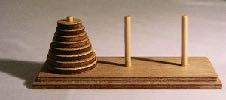
\includegraphics[scale=0.9]{hanoi.jpg}
\end{figure}
O objetivo do jogo é trazer todos os discos da haste esquerda para a haste
direita seguindo as seguintes três regras simples:
\begin{enumerate}
\item Apenas um disco pode ser movido por vez;
\item Cada movimento consiste em retirar o disco que está mais acima em uma das hastes, e o colocar no topo de outra haste;
\item Nenhum disco pode ser colocado sobre um disco menor;
\end{enumerate}
Seu objetivo é criar um simulador da solução mais otimizada para este
puzzle.
\newline \newline
\textbf{{\large Entrada}} \newline
A entrada consiste de apenas dois inteiros \textbf{H} e \textbf{P}, descrevendo o número de
discos da torre de Hanoi e o número de passos desejados, respectivamente.
\newline \newline
\textbf{{\large Saída}} \newline
Seu programa deve simular a solução ótima do puzzle e parar após a
execução de \textbf{P} passos. Ao final da execução, ele deve imprimir na saída
padrão três inteiros, cada um descrevendo a quantidade de discos em cada
torre após \textbf{P} passos.
\newline
\begin{table}[H]
\centering
\begin{tabular}{|l|l|}
\hline
\textbf{Exemplo de Entrada} & \textbf{Exemplo de Saída} \\ \hline
4 3                         & 2 0 2                     \\ \hline
3 1                         & 2 0 1                     \\ \hline
\end{tabular}
\caption{Questão G}
\label{tabela7}
\end{table}
\end{document}